% Options for packages loaded elsewhere
\PassOptionsToPackage{unicode}{hyperref}
\PassOptionsToPackage{hyphens}{url}
%
\documentclass[
  ignorenonframetext,
]{beamer}
\usepackage{pgfpages}
\setbeamertemplate{caption}[numbered]
\setbeamertemplate{caption label separator}{: }
\setbeamercolor{caption name}{fg=normal text.fg}
\beamertemplatenavigationsymbolsempty
% Prevent slide breaks in the middle of a paragraph
\widowpenalties 1 10000
\raggedbottom
\setbeamertemplate{part page}{
  \centering
  \begin{beamercolorbox}[sep=16pt,center]{part title}
    \usebeamerfont{part title}\insertpart\par
  \end{beamercolorbox}
}
\setbeamertemplate{section page}{
  \centering
  \begin{beamercolorbox}[sep=12pt,center]{part title}
    \usebeamerfont{section title}\insertsection\par
  \end{beamercolorbox}
}
\setbeamertemplate{subsection page}{
  \centering
  \begin{beamercolorbox}[sep=8pt,center]{part title}
    \usebeamerfont{subsection title}\insertsubsection\par
  \end{beamercolorbox}
}
\AtBeginPart{
  \frame{\partpage}
}
\AtBeginSection{
  \ifbibliography
  \else
    \frame{\sectionpage}
  \fi
}
\AtBeginSubsection{
  \frame{\subsectionpage}
}
\usepackage{amsmath,amssymb}
\usepackage{iftex}
\ifPDFTeX
  \usepackage[T1]{fontenc}
  \usepackage[utf8]{inputenc}
  \usepackage{textcomp} % provide euro and other symbols
\else % if luatex or xetex
  \usepackage{unicode-math} % this also loads fontspec
  \defaultfontfeatures{Scale=MatchLowercase}
  \defaultfontfeatures[\rmfamily]{Ligatures=TeX,Scale=1}
\fi
\usepackage{lmodern}
\usetheme[]{metropolis}
\usecolortheme{seahorse}
\ifPDFTeX\else
  % xetex/luatex font selection
\fi
% Use upquote if available, for straight quotes in verbatim environments
\IfFileExists{upquote.sty}{\usepackage{upquote}}{}
\IfFileExists{microtype.sty}{% use microtype if available
  \usepackage[]{microtype}
  \UseMicrotypeSet[protrusion]{basicmath} % disable protrusion for tt fonts
}{}
\makeatletter
\@ifundefined{KOMAClassName}{% if non-KOMA class
  \IfFileExists{parskip.sty}{%
    \usepackage{parskip}
  }{% else
    \setlength{\parindent}{0pt}
    \setlength{\parskip}{6pt plus 2pt minus 1pt}}
}{% if KOMA class
  \KOMAoptions{parskip=half}}
\makeatother
\usepackage{xcolor}
\newif\ifbibliography
\usepackage{graphicx}
\makeatletter
\def\maxwidth{\ifdim\Gin@nat@width>\linewidth\linewidth\else\Gin@nat@width\fi}
\def\maxheight{\ifdim\Gin@nat@height>\textheight\textheight\else\Gin@nat@height\fi}
\makeatother
% Scale images if necessary, so that they will not overflow the page
% margins by default, and it is still possible to overwrite the defaults
% using explicit options in \includegraphics[width, height, ...]{}
\setkeys{Gin}{width=\maxwidth,height=\maxheight,keepaspectratio}
% Set default figure placement to htbp
\makeatletter
\def\fps@figure{htbp}
\makeatother
\setlength{\emergencystretch}{3em} % prevent overfull lines
\providecommand{\tightlist}{%
  \setlength{\itemsep}{0pt}\setlength{\parskip}{0pt}}
\setcounter{secnumdepth}{-\maxdimen} % remove section numbering
\usepackage{xcolor}
\definecolor{myorange}{RGB}{255, 94, 77}
\setbeamertemplate{footline}{}
\ifLuaTeX
  \usepackage{selnolig}  % disable illegal ligatures
\fi
\IfFileExists{bookmark.sty}{\usepackage{bookmark}}{\usepackage{hyperref}}
\IfFileExists{xurl.sty}{\usepackage{xurl}}{} % add URL line breaks if available
\urlstyle{same}
\hypersetup{
  pdftitle={Introduction to Quantitative Reasoning I},
  pdfauthor={Professors David Ruth and David Puelz},
  hidelinks,
  pdfcreator={LaTeX via pandoc}}

\title{Introduction to Quantitative Reasoning I}
\author{Professors David Ruth and David Puelz}
\date{}
\institute{The University of Austin}

\begin{document}
\frame{\titlepage}

\begin{frame}{Introduction}
\protect\hypertarget{introduction}{}
\begin{itemize}
\tightlist
\item
  About your instructors
\item
  About the course
\end{itemize}
\end{frame}

\begin{frame}{Quantitative Reasoning I is\ldots{}}
\protect\hypertarget{quantitative-reasoning-i-is}{}
\ldots the first of a two-course sequence in quantitative reasoning.

Topics include interpretation of graphical information, functional
notation, patterns, mathematical problem formulation.

Throughout the course examples will be drawn from a variety of fields
including physics, biology, and economics; there will be particular
emphasis on the laws of nature and analogies among them.
\end{frame}

\begin{frame}{Course administration and syllabus}
\protect\hypertarget{course-administration-and-syllabus}{}
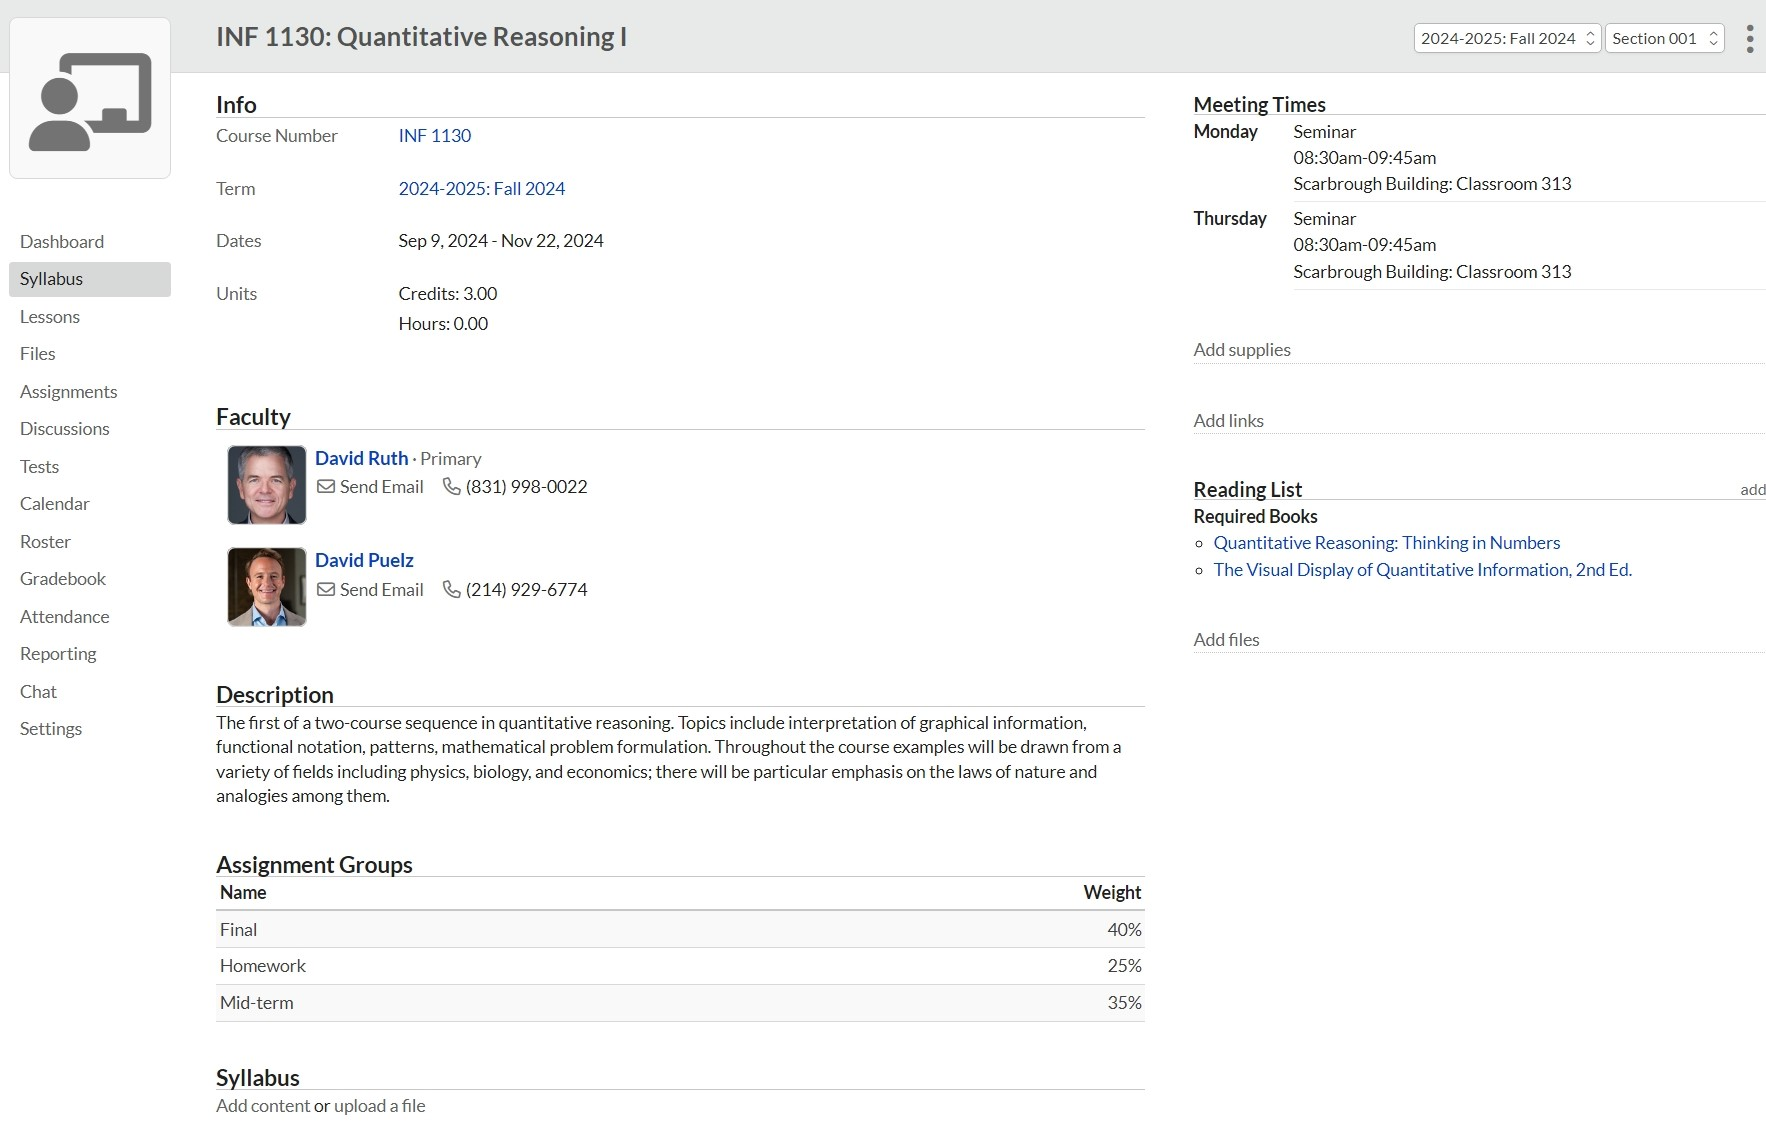
\includegraphics{"intro_figs/Populi1.jpeg"}
\end{frame}

\begin{frame}{Introduction to Visual Display of Quantitative
Information}
\protect\hypertarget{introduction-to-visual-display-of-quantitative-information}{}
\begingroup
\fontfamily{phv}\fontsize{16}{18}\selectfont
\begin{center}
  SEE TABLE HANDOUTS
\end{center}
\endgroup
\end{frame}

\begin{frame}{Table 1}
\protect\hypertarget{table-1}{}
\begin{figure}
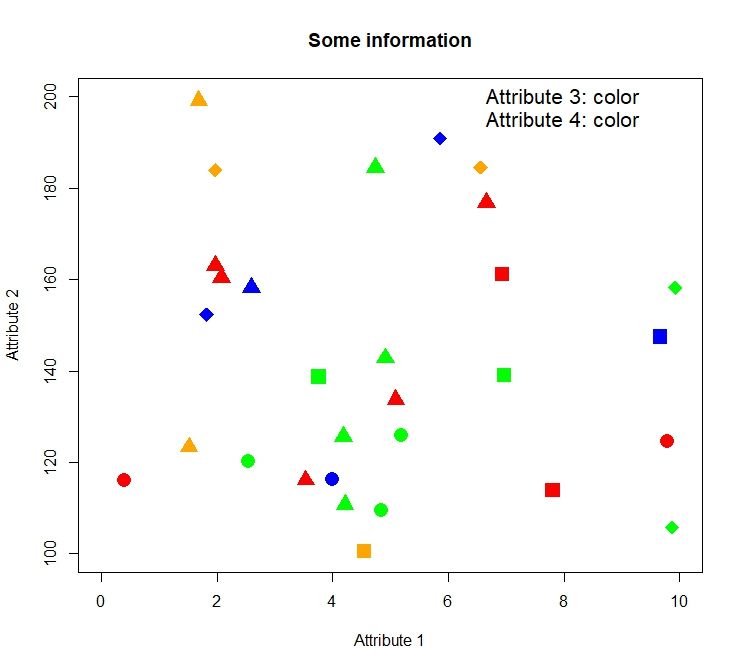
\includegraphics[width=0.85\linewidth]{intro_figs/tab1} \caption{Data from Table 1.}\label{fig:unnamed-chunk-1}
\end{figure}
\end{frame}

\begin{frame}{Table 2}
\protect\hypertarget{table-2}{}
\begin{figure}
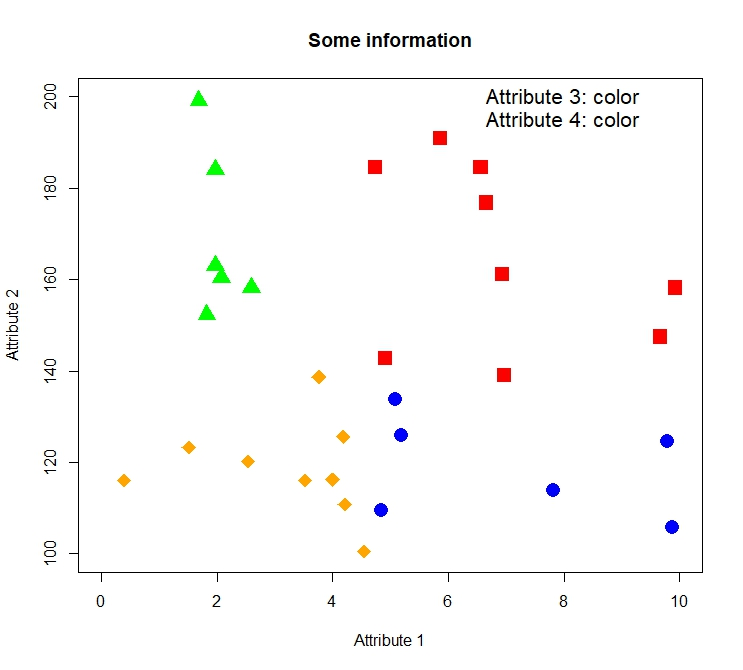
\includegraphics[width=0.85\linewidth]{intro_figs/tab2} \caption{Data from Table 2.}\label{fig:unnamed-chunk-2}
\end{figure}
\end{frame}

\begin{frame}{Table 3}
\protect\hypertarget{table-3}{}
\begin{figure}
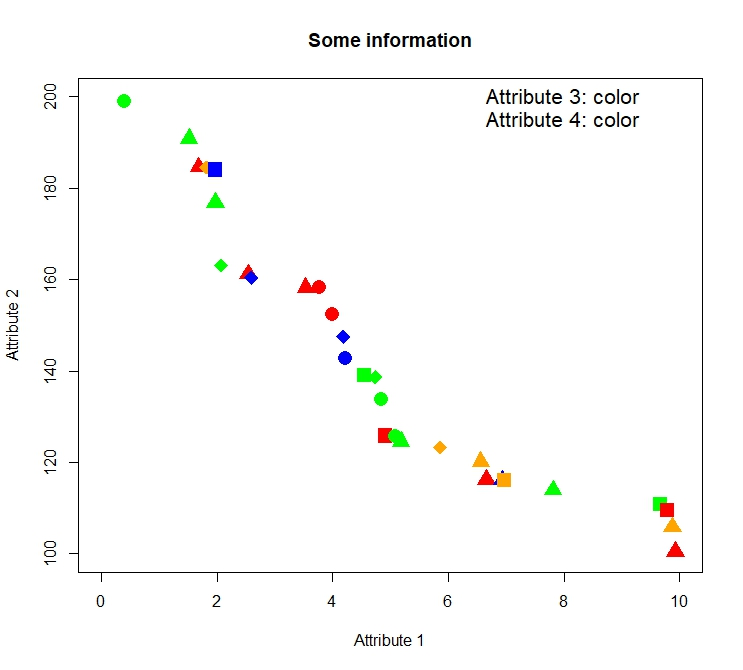
\includegraphics[width=0.85\linewidth]{intro_figs/tab3} \caption{Data from Table 3.}\label{fig:unnamed-chunk-3}
\end{figure}
\end{frame}

\end{document}
